\chapter{Cinética química: leyes de velocidad}\label{ch:b1:rate-laws}

La leche se conserva una semana en el frigorífico y un día sobre una mesa
en verano. La caja de un medicamento dice ``consérvese por debajo de
\qty{25}{\celsius}'' y lleva una fecha de caducidad a dos o tres años
vista, que el fabricante no tuvo tiempo de observar directamente. Las
constantes de equilibrio dicen dónde acaba una reacción; no dicen nada de
cuánto tarda en llegar allí. Ese es el dominio de la cinética química.
Este capítulo define la velocidad de una reacción, las \omterm{def:b1:rate-laws:order}{leyes de velocidad}
que la expresan en función de las concentraciones, las formas integradas
que predicen las concentraciones en cualquier instante, los métodos
experimentales que determinan una \omterm{def:b1:rate-laws:order}{ley de velocidad} y la \omterm{thm:b1:rate-laws:arrhenius}{ley de Arrhenius},
que describe el efecto de la temperatura --- la herramienta con la que se
predice en unas pocas semanas de experimentos la vida útil de un
medicamento.

\begin{recall}
El libro 1 (año 12) introdujo la velocidad de aparición y de desaparición
de una especie, los factores cinéticos (concentración, temperatura,
catalizador) y el \omterm{def:b1:rate-laws:half-life}{tiempo de semirreacción} de una reacción de primer
orden. El avance $\xi$ de una reacción se definió en la
\cref{def:b1:extent-q-and-k:extent}.
\end{recall}

\begin{omfigure}
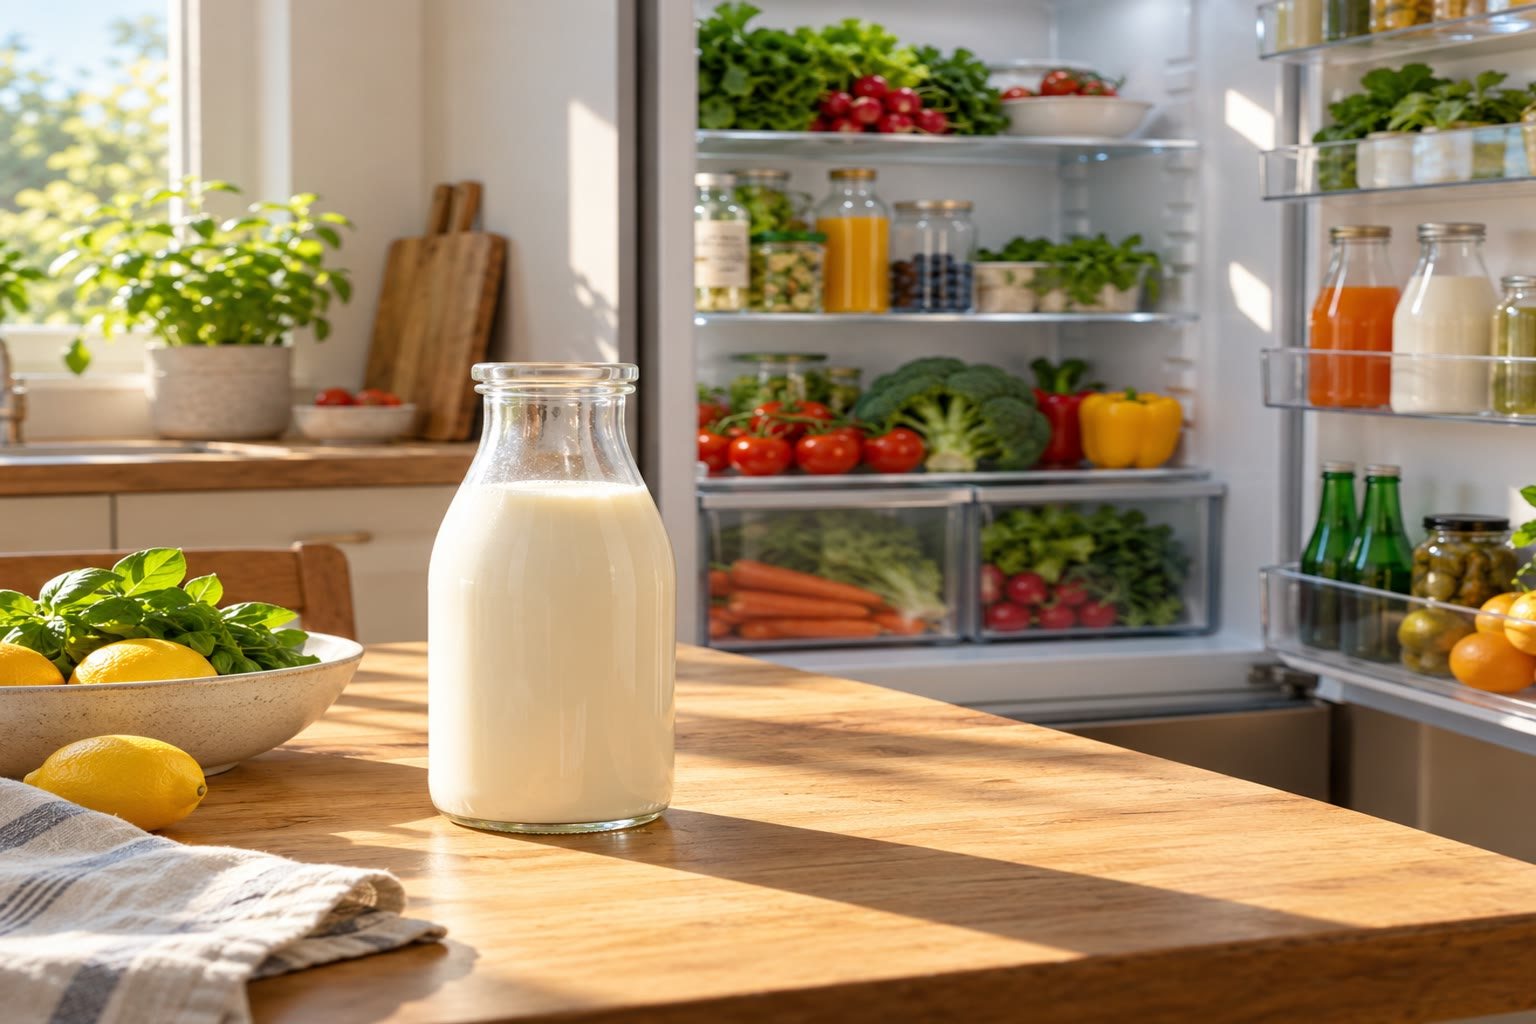
\includegraphics[width=0.55\linewidth]{images/book2/ai/b1-08-milk-kitchen.jpg}

{\small Una botella de leche al sol junto a un frigorífico abierto. Las
reacciones que la estropean van varias veces más deprisa a la temperatura
del verano que en el frío.}
\end{omfigure}

\section{La velocidad de una reacción}

\begin{definition}[Velocidad de reacción, velocidades de formación y de desaparición]\label{def:b1:rate-laws:rate}
Para una reacción $0 = \sum_i \nu_i\mathrm{A}_i$ que tiene lugar en un
reactor cerrado de volumen constante $V$, la \emph{velocidad de
reacción}\index{velocidad de reaccion@velocidad de reacción} es
\[
  v = \frac{1}{V}\frac{\dd\xi}{\dd t} = \frac{1}{\nu_i}\frac{\dd[\mathrm{A}_i]}{\dd t}
  \quad\text{(cualquier } i\text{)},
\]
en \unit{mol.L^{-1}.s^{-1}}. La \emph{velocidad de formación}\index{velocidad de formacion@velocidad de formación}
de un producto es $\dd[\mathrm{A}_i]/\dd t$; la \emph{velocidad de
desaparición}\index{velocidad de desaparicion@velocidad de desaparición} de un reactivo es
$-\dd[\mathrm{A}_i]/\dd t$.
\end{definition}

\begin{proposition}[Una sola velocidad para todas las especies]\label{prop:b1:rate-laws:rate-relations}
La \omterm{def:b1:rate-laws:rate}{velocidad de reacción} no depende de la especie elegida para seguirla:
para $a\,\mathrm{A} + b\,\mathrm{B} \longrightarrow c\,\mathrm{C} + d\,\mathrm{D}$,
\[
  v = -\frac1a\frac{\dd[\ce{A}]}{\dd t} = -\frac1b\frac{\dd[\ce{B}]}{\dd t}
  = \frac1c\frac{\dd[\ce{C}]}{\dd t} = \frac1d\frac{\dd[\ce{D}]}{\dd t} .
\]
\end{proposition}

\begin{proof}
$[\mathrm{A}_i] = (n_{i,0} + \nu_i\xi)/V$ con $V$ constante, de modo que
$\dd[\mathrm{A}_i]/\dd t = (\nu_i/V)\,\dd\xi/\dd t = \nu_i v$.
\end{proof}

\begin{example}[Descomposición del pentóxido de dinitrógeno]\label{ex:b1:rate-laws:n2o5}
Para \ce{2N2O5 -> 4NO2 + O2}: $v = -\frac12\frac{\dd[\ce{N2O5}]}{\dd t} =
\frac14\frac{\dd[\ce{NO2}]}{\dd t} = \frac{\dd[\ce{O2}]}{\dd t}$. El
dióxido de nitrógeno aparece cuatro veces más deprisa que el dioxígeno, y
el pentóxido de dinitrógeno desaparece el doble de deprisa de lo que
aparece el dioxígeno.
\end{example}

\section{Leyes de velocidad y órdenes}

\begin{definition}[Ley de velocidad, órdenes, constante de velocidad]\label{def:b1:rate-laws:order}
Una \emph{ley de velocidad}\index{ley de velocidad} expresa la velocidad en
función de las concentraciones. Una reacción \emph{admite un orden} cuando
su ley de velocidad es de la forma
\[
  v = k\,[\mathrm{A}]^{p}\,[\mathrm{B}]^{q} \cdots ;
\]
los exponentes $p$, $q$, \dots\ son los \emph{órdenes parciales}\index{orden parcial}
respecto de A, B, \dots; su suma es el \emph{orden
global}\index{orden global}, y $k$ es la \emph{constante de velocidad}\index{constante de velocidad},
que solo depende de la temperatura. Los órdenes se determinan
experimentalmente; no tienen por qué coincidir con los coeficientes
estequiométricos, y pueden ser fraccionarios o nulos.
\end{definition}

\begin{remark}[Unidades de $k$]\label{rem:b1:rate-laws:units}
Como $v$ se expresa en \unit{mol.L^{-1}.s^{-1}}, $k$ se expresa en
\unit{mol.L^{-1}.s^{-1}} para el orden 0, en \unit{s^{-1}} para el orden
1, en \unit{L.mol^{-1}.s^{-1}} para el orden 2 y, en general, en
$(\unit{mol/L})^{1-n}\,\unit{s^{-1}}$ para el \omterm{def:b1:rate-laws:order}{orden global} $n$. La unidad
de $k$ indica el \omterm{def:b1:rate-laws:order}{orden global}.
\end{remark}

\begin{remark}[Reacciones sin orden]\label{rem:b1:rate-laws:no-order}
No toda reacción admite un orden. La velocidad de algunas reacciones es
una fracción cuyo denominador contiene concentraciones, o depende de la
concentración de un producto. Tales \omterm{def:b1:rate-laws:order}{leyes de velocidad} se explican por el
mecanismo de la reacción (\cref{ch:b1:elementary-steps}). Una reacción
también puede admitir un orden solo al principio: la ley de \omterm{def:b1:rate-laws:initial-rate}{velocidad
inicial}.
\end{remark}

\section{Leyes de velocidad integradas y tiempos de semirreacción}

\begin{definition}[Tiempo de semirreacción]\label{def:b1:rate-laws:half-life}
El \emph{tiempo de semirreacción}\index{tiempo de semirreaccion@tiempo de semirreacción} $t_{1/2}$ de un
reactivo es el tiempo al cabo del cual se ha consumido la mitad de su
cantidad inicial.
\end{definition}

\begin{theorem}[Leyes de velocidad integradas]\label{thm:b1:rate-laws:integrated}
Para una reacción $a\mathrm{A} \rightarrow \text{productos}$ de velocidad $v = -\frac1a\frac{\dd[\ce{A}]}
{\dd t} = k[\ce{A}]^n$, con $[\ce{A}](0) = a_0$:
\begin{center}
\begin{tabular}{llll}
\hline
orden & ley integrada & representación lineal & \omterm{def:b1:rate-laws:half-life}{tiempo de semirreacción} \\
\hline
0 & $[\ce{A}] = a_0 - akt$ & $[\ce{A}]$ frente a $t$ & $a_0/(2ak)$ \\
1 & $[\ce{A}] = a_0\,\eu^{-akt}$ & $\ln[\ce{A}]$ frente a $t$ & $\ln2/(ak)$ \\
2 & $\dfrac{1}{[\ce{A}]} = \dfrac{1}{a_0} + akt$ & $1/[\ce{A}]$ frente a $t$ & $1/(ak\,a_0)$ \\
\hline
\end{tabular}
\end{center}
\end{theorem}

\begin{proof}
Sea $c = [\ce{A}]$, de modo que $\dd c/\dd t = -akc^n$.
\emph{Orden 0}: $\dd c/\dd t = -ak$, luego $c = a_0 - akt$ (válida hasta
que $c = 0$). \emph{Orden 1}: $\dd c/\dd t = -akc$ es una ecuación
diferencial lineal de primer orden cuya solución es $c = a_0\eu^{-akt}$.
\emph{Orden 2}: $\dd c/c^2 = -ak\,\dd t$; al integrar de 0 a $t$,
$-1/c + 1/a_0 = -akt$, de modo que $1/c = 1/a_0 + akt$. \omterm{def:b1:rate-laws:half-life}{Tiempos de
semirreacción}: se toma $c =
a_0/2$ en cada ley y se despeja $t$.
\end{proof}

\begin{proposition}[La prueba del tiempo de semirreacción]\label{prop:b1:rate-laws:half-life-test}
El \omterm{def:b1:rate-laws:half-life}{tiempo de semirreacción} es independiente de la concentración inicial
si y solo si la reacción es de orden 1. Es proporcional a $a_0$ para el
orden 0 y a $1/a_0$ para el orden 2. Una reacción de primer orden pierde
la mitad de lo que queda en cada \omterm{def:b1:rate-laws:half-life}{tiempo de semirreacción} sucesivo: al
cabo de $m$ \omterm{def:b1:rate-laws:half-life}{tiempos de semirreacción} queda una fracción $2^{-m}$.
\end{proposition}

\begin{proof}
Para el orden $n \ne 1$, la separación de variables da $t_{1/2} = \dfrac{2^{n-1} -
1}{(n-1)\,ak\,a_0^{n-1}}$, que depende de $a_0$ salvo si $n = 1$; para
$n = 1$, $t_{1/2} = \ln2/(ak)$. Para el orden 1, $c(t + t_{1/2}) = c(t)/2$
en todo instante $t$, ya que $\eu^{-ak(t + t_{1/2})} = \eu^{-akt}/2$.
\end{proof}

\begin{omfigure}
\begin{tikzpicture}
\begin{axis}[name=p0,
  width=0.36\linewidth, height=4.6cm,
  xmin=0, xmax=60, ymin=0, ymax=1.05,
  axis x line=bottom, axis y line=left,
  xlabel={$t$ (min)}, title={orden 0: $[\ce{A}]$},
  title style={font=\small}, xtick={0,20,40,60},
  tick label style={font=\scriptsize}, label style={font=\small}]
\addplot[omDef, thick] table[x=t, y=A0] {figdata/out/bachelor-1-integrated-rate-laws.dat};
\end{axis}
\begin{axis}[at={(p0.east)}, anchor=west, xshift=0.9cm, name=p1,
  width=0.36\linewidth, height=4.6cm,
  xmin=0, xmax=60, ymin=-3.2, ymax=0.2,
  axis x line=bottom, axis y line=left,
  xlabel={$t$ (min)}, title={orden 1: $\ln[\ce{A}]$},
  title style={font=\small}, xtick={0,20,40,60},
  tick label style={font=\scriptsize}, label style={font=\small}]
\addplot[omProp, thick] table[x=t, y=lnA1] {figdata/out/bachelor-1-integrated-rate-laws.dat};
\end{axis}
\begin{axis}[at={(p1.east)}, anchor=west, xshift=0.9cm,
  width=0.36\linewidth, height=4.6cm,
  xmin=0, xmax=60, ymin=0, ymax=4.2,
  axis x line=bottom, axis y line=left,
  xlabel={$t$ (min)}, title={orden 2: $1/[\ce{A}]$},
  title style={font=\small}, xtick={0,20,40,60},
  tick label style={font=\scriptsize}, label style={font=\small}]
\addplot[omThm, thick] table[x=t, y=invA2] {figdata/out/bachelor-1-integrated-rate-laws.dat};
\end{axis}
\end{tikzpicture}

\begin{tikzpicture}
\begin{axis}[
  width=0.62\linewidth, height=5.0cm,
  xmin=0, xmax=60, ymin=0, ymax=1.05,
  axis x line=bottom, axis y line=left,
  xlabel={$t$ (min)}, ylabel={$[\ce{A}]$ (mol/L)}, xtick={0,10,20,30,40,50,60},
  tick label style={font=\small}, label style={font=\small},
  legend style={font=\small, draw=none, at={(0.98,0.98)}, anchor=north east}]
\addplot[omDef, thick] table[x=t, y=A0] {figdata/out/bachelor-1-integrated-rate-laws.dat};
\addplot[omProp, thick] table[x=t, y=A1] {figdata/out/bachelor-1-integrated-rate-laws.dat};
\addplot[omThm, thick] table[x=t, y=A2] {figdata/out/bachelor-1-integrated-rate-laws.dat};
\legend{orden 0, orden 1, orden 2}
\draw[dotted] (axis cs:0,0.5) -- (axis cs:20,0.5);
\end{axis}
\end{tikzpicture}

{\small Tres reacciones con la misma concentración inicial
(\qty{1.00}{mol/L}) y la misma \omterm{def:b1:rate-laws:initial-rate}{velocidad inicial}
(\qty{0.050}{mol.L^{-1}.min^{-1}}). Arriba, cada ley integrada se
convierte en una recta en sus propias coordenadas. Abajo, las
concentraciones; los \omterm{def:b1:rate-laws:half-life}{tiempos de semirreacción} son 10, 13.9 y 20 minutos.}
\end{omfigure}

\section{Determinar una ley de velocidad}

\begin{method}[El método integral]\label{met:b1:rate-laws:integral}
Para probar un orden con medidas de $[\ce{A}](t)$: se representan
$[\ce{A}]$, $\ln[\ce{A}]$ y $1/[\ce{A}]$ frente a $t$; la representación
que es una recta da el orden, y su pendiente da $k$ (pendiente $-ak$,
$-ak$ o $+ak$, respectivamente).
\end{method}

\begin{method}[El método del tiempo de semirreacción]\label{met:b1:rate-laws:half-life}
Se mide el \omterm{def:b1:rate-laws:half-life}{tiempo de semirreacción} para varias concentraciones iniciales:
constante, orden 1; proporcional a $a_0$, orden 0; proporcional a
$1/a_0$, orden 2. En un solo experimento, se comparan los tiempos que se
tarda en pasar de $a_0$ a $a_0/2$ y de $a_0/2$ a $a_0/4$: tiempos iguales
indican orden 1.
\end{method}

\begin{definition}[Velocidad inicial]\label{def:b1:rate-laws:initial-rate}
La \emph{velocidad inicial}\index{velocidad inicial} $v_0$ es la velocidad
en $t = 0$, leída como la pendiente de la tangente en el origen de la
curva $[\ce{A}](t)$, dividida por el coeficiente estequiométrico. En ese
momento las concentraciones son las iniciales, conocidas, y ningún
producto interfiere.
\end{definition}

\begin{method}[El método de las velocidades iniciales]\label{met:b1:rate-laws:initial-rates}
Para $v_0 = k[\ce{A}]_0^p[\ce{B}]_0^q$: se realizan experimentos en los
que solo cambia $[\ce{A}]_0$; entonces, $\ln v_0 = \ln(k[\ce{B}]_0^q) + p\ln[\ce{A}]_0$,
y la pendiente de $\ln v_0$ frente a $\ln[\ce{A}]_0$ es $p$. En la
práctica, duplicar $[\ce{A}]_0$ multiplica $v_0$ por $2^p$. Se procede
igual con B.
\end{method}

\begin{definition}[Método de aislamiento, orden aparente]\label{def:b1:rate-laws:apparent-order}
En el \emph{método de aislamiento}\index{metodo de aislamiento@método de aislamiento}, todos los
reactivos salvo uno se ponen en gran exceso (diez veces o más). Sus
concentraciones permanecen prácticamente constantes, y $v = k[\ce{A}]^p[\ce{B}]^q \approx k'[\ce{A}]^p$
con $k' = k[\ce{B}]_0^q$: la reacción se comporta como si fuera de
\emph{orden aparente}\index{orden aparente} $p$, con la \omterm{def:b1:rate-laws:order}{constante de
velocidad} aparente $k'$. También se habla de degeneración del orden.
\end{definition}

\begin{omfigure}
\begin{tikzpicture}
\begin{axis}[
  width=0.55\linewidth, height=4.8cm,
  xmin=0, xmax=40, ymin=0, ymax=1.05,
  axis x line=bottom, axis y line=left,
  xlabel={$t$ (min)}, ylabel={$[\ce{A}]$ (mol/L)},
  xtick={0,10,20,30,40},
  tick label style={font=\small}, label style={font=\small}, clip mode=individual]
\addplot[omProp, thick] table[x=t, y=A1] {figdata/out/bachelor-1-integrated-rate-laws.dat};
\draw[omThm, thick] (axis cs:0,1) -- (axis cs:20,0);
\node[omThm, anchor=west, font=\small] at (axis cs:2,0.12) {tangente en $t = 0$};
\end{axis}
\end{tikzpicture}

{\small Lectura de una \omterm{def:b1:rate-laws:initial-rate}{velocidad inicial}: la tangente en el origen (en
rojo) de una curva de primer orden corta el eje de tiempos en
$t_0 = \qty{20}{min}$, de modo que $v_0 =
\qty{1.00}{mol/L}/\qty{20}{min} = \qty{0.050}{mol.L^{-1}.min^{-1}}$.}
\end{omfigure}

\begin{inthelab}[Seguir una reacción en el tiempo]
Una \omterm{def:b1:rate-laws:order}{ley de velocidad} se construye con concentraciones medidas mientras la
reacción transcurre. Cuando un reactivo o un producto es coloreado, un
espectrofotómetro registra la absorbancia, proporcional a su
concentración (Beer--Lambert, \cref{ch:b1:structure-spectroscopy});
cuando aparecen o desaparecen iones, un conductímetro sigue la
conductividad; cuando se forma un gas en un recipiente cerrado, un
manómetro sigue la presión. En otro caso, se toman muestras en instantes
conocidos, se detiene la reacción (se bloquea) por enfriamiento o por
dilución y se valora cada muestra. La temperatura del recipiente se
mantiene constante con un baño termostático, porque $k$ depende mucho de
ella.
\end{inthelab}

\section{La temperatura: la ley de Arrhenius}

\begin{definition}[Energía de activación]\label{def:b1:rate-laws:activation-energy}
La \emph{energía de activación}\index{energia de activacion@energía de activación} $E_a$ de una
reacción de \omterm{def:b1:rate-laws:order}{constante de velocidad} $k(T)$ se define mediante
\[
  \frac{\dd \ln k}{\dd T} = \frac{E_a}{RT^2} ,
\]
en \unit{J/mol}. Cuando $E_a$ es independiente de $T$, la integración da
$k = A\,\eu^{-E_a/RT}$, donde la constante $A$, de la misma unidad que
$k$, es el \emph{factor preexponencial}\index{factor preexponencial}.
\end{definition}

\begin{theorem}[Ley de Arrhenius]\label{thm:b1:rate-laws:arrhenius}
Para la mayoría de las reacciones, en un intervalo de temperatura
moderado, la \omterm{def:b1:rate-laws:order}{constante de velocidad} sigue la \emph{ley de
Arrhenius}\index{ley de Arrhenius}
\[
  k(T) = A\,\eu^{-E_a/RT} ,
\]
con $A$ y $E_a > 0$ independientes de $T$: $\ln k$ es una función lineal
de $1/T$ de pendiente $-E_a/R$.
\end{theorem}
\admitted

\begin{remark}[El significado de $E_a$]\label{rem:b1:rate-laws:meaning}
La ley es empírica. Su interpretación --- solo conducen a la reacción los
choques moleculares que aportan al menos una energía del orden de $E_a$,
y la fracción de tales choques varía como $\eu^{-E_a/RT}$ --- se esboza
con los perfiles de energía del capítulo siguiente, y la hacen
cuantitativa las teorías de la \omterm{def:b1:rate-laws:rate}{velocidad de reacción} en el volumen del
tercer año.
\end{remark}

\begin{method}[Determinar $E_a$]\label{met:b1:rate-laws:arrhenius-plot}
A partir de \omterm{def:b1:rate-laws:order}{constantes de velocidad} a varias temperaturas, se representa
$\ln k$ frente a $1/T$ (en kelvin): la pendiente es $-E_a/R$, y la
ordenada en el origen, $\ln A$. Con solo dos temperaturas,
\[
  E_a = \frac{R\,\ln(k_2/k_1)}{1/T_1 - 1/T_2} .
\]
\end{method}

\begin{example}[Una regla práctica]\label{ex:b1:rate-laws:doubling}
Para $E_a = \qty{53}{kJ/mol}$, pasar de 25 a \qty{35}{\celsius} multiplica
$k$ por $\exp\!\big(\frac{53000}{8.314}(\frac{1}{298.15} -
\frac{1}{308.15})\big) = 2.0$. La conocida regla ``diez grados más, el
doble de rápido'' se cumple cerca de la temperatura ambiente para
reacciones de \omterm{def:b1:rate-laws:activation-energy}{energía de activación} en torno a \qty{50}{kJ/mol}; para
$E_a$ mayores, el factor es mayor.
\end{example}

\begin{omfigure}
\begin{tikzpicture}
\begin{axis}[
  width=0.6\linewidth, height=5.4cm,
  xmin=2.95, xmax=3.45, ymin=-9.0, ymax=-4.2, clip mode=individual,
  axis x line=bottom, axis y line=left,
  xlabel={$1000/T$ (\unit{K^{-1}})}, ylabel={$\ln k$ ($k$ en \unit{d^{-1}})},
  xtick={3.0,3.1,3.2,3.3,3.4}, ytick={-9,-8,-7,-6,-5},
  tick label style={font=\small}, label style={font=\small}]
\addplot[omDef, thick] table[x=invT_1e3, y=lnk] {figdata/out/bachelor-1-arrhenius-line.dat};
\addplot[only marks, mark=*, mark size=2.2pt, omThm] table[x=invT_1e3, y=lnk] {figdata/out/bachelor-1-arrhenius-points.dat};
\node[font=\small, anchor=south west] at (axis cs:3.002,-4.71) {\qty{60}{\celsius}};
\node[font=\small, anchor=south west] at (axis cs:3.095,-5.66) {\qty{50}{\celsius}};
\node[font=\small, anchor=south west] at (axis cs:3.193,-6.67) {\qty{40}{\celsius}};
\draw[dashed, black!50] (axis cs:3.354,-9.0) -- (axis cs:3.354,-8.31);
\addplot[only marks, mark=o, mark size=2.4pt, omDef] coordinates {(3.354,-8.310)};
\node[font=\small, anchor=east] at (axis cs:3.33,-8.40) {\qty{25}{\celsius}, extrapolado};
\end{axis}
\end{tikzpicture}

{\small Representación de Arrhenius de la degradación de un medicamento
(problema de fin de semana): tres \omterm{def:b1:rate-laws:order}{constantes de velocidad} medidas (en
rojo) están sobre una recta de pendiente $-E_a/R$; extrapolada a
\qty{25}{\celsius}, da la vida útil a temperatura ambiente.}
\end{omfigure}

\begin{history}[Arrhenius, 1889]
El químico sueco Svante Arrhenius, al estudiar en 1889 la inversión de la
sacarosa por los ácidos, propuso que solo reacciona una pequeña fracción
de las moléculas, las que están en un estado ``activado'', y que esta
fracción crece con la temperatura como $\eu^{-E/RT}$. La idea, polémica al
principio, se convirtió en el fundamento de la cinética química. Arrhenius
recibió el Premio Nobel de Química en 1903, por su teoría de la
disociación electrolítica.
\end{history}

\begin{omfigure}
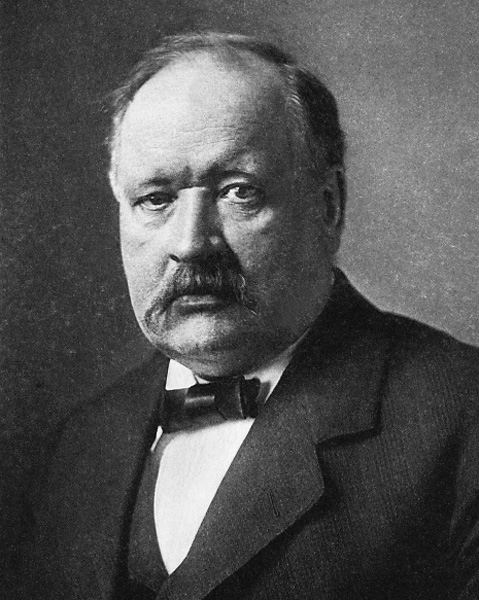
\includegraphics[width=0.22\linewidth]{images/book2/arrhenius.jpg}

{\small Svante Arrhenius (1859--1927), en 1909.}
\end{omfigure}

\section{Ejercicios}

\begin{exercise}[$\star$]\label{exo:b1:rate-laws:1}
Para \ce{2N2O5 -> 4NO2 + O2} a volumen constante, el dióxido de nitrógeno
aparece a $\qty{2.0e-4}{mol.L^{-1}.s^{-1}}$. Dense la \omterm{def:b1:rate-laws:rate}{velocidad de
reacción}, la \omterm{def:b1:rate-laws:rate}{velocidad de formación} del dioxígeno y la \omterm{def:b1:rate-laws:rate}{velocidad de
desaparición} de \ce{N2O5}.
\end{exercise}

\begin{exercise}[$\star$]\label{exo:b1:rate-laws:2}
Dese la unidad de la \omterm{def:b1:rate-laws:order}{constante de velocidad} para los \omterm{def:b1:rate-laws:order}{órdenes globales} 0,
1, 2 y 3, con las concentraciones en \unit{mol/L} y los tiempos en
segundos.
\end{exercise}

\begin{exercise}[$\star$]\label{exo:b1:rate-laws:3}
Una reacción de primer orden $\mathrm{A} \longrightarrow \mathrm{B}$ tiene
$k = \qty{3.0e-3}{s^{-1}}$. Calcúlense su \omterm{def:b1:rate-laws:half-life}{tiempo de semirreacción} y la
fracción de \ce{A} que queda al cabo de \qty{10}{min}.
\end{exercise}

\begin{exercise}[$\star$]\label{exo:b1:rate-laws:4}
Cuando la concentración inicial de un reactivo se divide por dos, su
\omterm{def:b1:rate-laws:half-life}{tiempo de semirreacción} se duplica. ¿Cuál es el orden? ¿Y si el \omterm{def:b1:rate-laws:half-life}{tiempo de
semirreacción} se divide por dos?
\end{exercise}

\begin{exercise}[$\star\star$]\label{exo:b1:rate-laws:5}
Se mide la concentración de un reactivo \ce{A} ($\mathrm{A} \longrightarrow \mathrm{P}$): en $t
= 0$, 10, 20, 30 y \qty{40}{min}, $[\ce{A}] = 0.100$, 0.0741, 0.0549,
0.0407 y \qty{0.0301}{mol/L}. Determínense el orden y la \omterm{def:b1:rate-laws:order}{constante de
velocidad}.
\end{exercise}

\begin{exercise}[$\star\star$]\label{exo:b1:rate-laws:6}
Para $\mathrm{A} + \mathrm{B} \longrightarrow \mathrm{P}$, $v_0 = \qty{2.0e-6}{mol.L^{-1}.s^{-1}}$ con $[\ce{A}]_0
= [\ce{B}]_0 = \qty{0.010}{mol/L}$; \qty{8.0e-6}{} cuando se duplica
$[\ce{A}]_0$; \qty{4.0e-6}{} cuando se duplica $[\ce{B}]_0$. Hállense los
\omterm{def:b1:rate-laws:order}{órdenes parciales}, la \omterm{def:b1:rate-laws:order}{ley de velocidad} y la \omterm{def:b1:rate-laws:order}{constante de velocidad}.
\end{exercise}

\begin{exercise}[$\star\star$]\label{exo:b1:rate-laws:7}
La \omterm{def:b1:rate-laws:order}{ley de velocidad} de $\mathrm{A} + \mathrm{B} \longrightarrow \mathrm{P}$ es $v = k[\ce{A}][\ce{B}]$. Con
$[\ce{B}]_0 = \qty{0.50}{mol/L}$ y $[\ce{A}]_0 = \qty{5.0e-3}{mol/L}$,
\ce{A} desaparece con una cinética de primer orden y una constante
aparente de \qty{0.012}{s^{-1}}. Explíquese y calcúlese $k$.
\end{exercise}

\begin{exercise}[$\star\star$]\label{exo:b1:rate-laws:8}
Una \omterm{def:b1:rate-laws:order}{constante de velocidad} vale \qty{1.0e-3}{s^{-1}} a \qty{300}{K} y
\qty{5.0e-3}{s^{-1}} a \qty{320}{K}. Calcúlense la \omterm{def:b1:rate-laws:activation-energy}{energía de activación} y
la \omterm{def:b1:rate-laws:order}{constante de velocidad} a \qty{310}{K}.
\end{exercise}

\begin{exercise}[$\star\star$]\label{exo:b1:rate-laws:9}
La reacción $2\,\mathrm{A} \longrightarrow \mathrm{P}$ tiene la \omterm{def:b1:rate-laws:order}{ley de velocidad} $v = -\frac12\frac{\dd[\ce{A}]}
{\dd t} = k[\ce{A}]^2$ con $k = \qty{0.50}{L.mol^{-1}.s^{-1}}$. Partiendo
de $[\ce{A}]_0 = \qty{0.020}{mol/L}$, calcúlense el \omterm{def:b1:rate-laws:half-life}{tiempo de
semirreacción} y la concentración al cabo de \qty{100}{s}.
\end{exercise}

\begin{exercise}[$\star\star\star$]\label{exo:b1:rate-laws:10}
Para una reacción de primer orden, demuéstrese que el tiempo necesario
para consumir una fracción $f$ del reactivo es $t_f = -\ln(1 - f)/(ak)$.
Compárense los tiempos para el 50\,\%, el 75\,\%, el 90\,\% y el
99.9\,\%, en \omterm{def:b1:rate-laws:half-life}{tiempos de semirreacción}.
\end{exercise}

\begin{exercise}[$\star\star\star$]\label{exo:b1:rate-laws:11}
Un parche cutáneo libera un fármaco a una velocidad constante de
\qty{0.40}{mg/h} mientras su depósito, inicialmente de \qty{10}{mg}, no
esté vacío. Escríbase la ley de la cantidad restante y dense su orden, su
\omterm{def:b1:rate-laws:half-life}{tiempo de semirreacción} y el tiempo al cabo del cual el parche se agota.
¿Por qué conviene una cinética de orden cero a un parche de fármaco?
\end{exercise}

\begin{exercise}[$\star\star\star$]\label{exo:b1:rate-laws:12}
Demuéstrese que la regla ``diez grados más, el doble de rápido'' entre
\qty{298.15}{K} y \qty{308.15}{K} corresponde a $E_a \approx
\qty{53}{kJ/mol}$. ¿Qué factor da la misma \omterm{def:b1:rate-laws:activation-energy}{energía de activación} entre
\qty{0}{\celsius} y \qty{10}{\celsius}?
\end{exercise}

\section{Problema: la vida útil de un medicamento}

\begin{problem}[{Problema de fin de semana --- un ensayo de estabilidad
acelerado: degradación de primer orden a 60\,\textdegree C, tres
temperaturas, la representación de Arrhenius y la vida útil a
temperatura ambiente}]
\label{pb:b1:rate-laws:1}
Para predecir la vida útil $t_{90}$ de un comprimido (el tiempo al cabo del
cual se ha degradado el 10\,\% del principio activo), un laboratorio
conserva muestras a temperatura elevada y mide el porcentaje de principio
activo que queda. A
\qty{60}{\celsius}:
\begin{center}
\begin{tabular}{lccccc}
\hline
tiempo (días) & 0 & 10 & 20 & 30 & 40 \\
principio activo restante (\%) & 100.0 & 91.4 & 83.5 & 76.3 & 69.8 \\
\hline
\end{tabular}
\end{center}
A 40 y \qty{50}{\celsius}, las \omterm{def:b1:rate-laws:order}{constantes de velocidad} halladas son
\qty{1.27e-3}{d^{-1}} y \qty{3.48e-3}{d^{-1}}. Tómense $R =
\qty{8.314}{J/(mol.K)}$ y un mes $= \qty{30.4}{d}$.

\medskip
\noindent\textbf{Parte I --- El orden a 60\,\textdegree C.}
\begin{enumerate}
  \item Calcúlense las pérdidas en cada intervalo de 10 días. ¿Es la
        reacción de orden 0?
  \item Calcúlese $\ln(\%\text{ restante})$ en cada instante. ¿Qué se
        concluye?
  \item Dedúzcase la \omterm{def:b1:rate-laws:order}{constante de velocidad} $k_{60}$.
  \item Calcúlese el \omterm{def:b1:rate-laws:half-life}{tiempo de semirreacción} a \qty{60}{\celsius}.
  \item ¿Qué porcentaje queda al cabo de 60 días a \qty{60}{\celsius}?
  \item Calcúlese $t_{90}$ a \qty{60}{\celsius}.
\end{enumerate}

\medskip
\noindent\textbf{Parte II --- Vida útil y orden.}
\begin{enumerate}[resume]
  \item Demuéstrese que, para una degradación de primer orden,
        $t_{90} = \ln(10/9)/k$.
  \item Exprésese $t_{90}$ como fracción del \omterm{def:b1:rate-laws:half-life}{tiempo de semirreacción}.
  \item ¿Por qué $t_{90}$ no depende de la dosis del comprimido?
  \item ¿Por qué los laboratorios miden la degradación a temperatura
        elevada y no a \qty{25}{\celsius}?
  \item Si la degradación fuera de orden 2 respecto del principio activo,
        ¿un comprimido del doble de dosis se conservaría más o menos
        tiempo? Explíquese.
\end{enumerate}

\medskip
\noindent\textbf{Parte III --- La representación de Arrhenius.}
\begin{enumerate}[resume]
  \item Tabúlense $1/T$ y $\ln k$ para las tres temperaturas.
  \item Calcúlese la pendiente de la recta que pasa por los puntos de 40 y
        \qty{60}{\celsius}.
  \item Dedúzcase la \omterm{def:b1:rate-laws:activation-energy}{energía de activación}.
  \item Compruébese que el punto de \qty{50}{\celsius} está sobre la
        recta.
  \item Calcúlese el \omterm{def:b1:rate-laws:activation-energy}{factor preexponencial} $A$.
  \item ¿En qué factor aumenta la velocidad entre 25 y
        \qty{35}{\celsius}? Compárese con la regla práctica.
\end{enumerate}

\medskip
\noindent\textbf{Parte IV --- La temperatura ambiente.}
\begin{enumerate}[resume]
  \item Extrapólese la \omterm{def:b1:rate-laws:order}{constante de velocidad} a \qty{30}{\celsius}.
  \item Calcúlese $t_{90}$ a \qty{30}{\celsius}, en meses.
  \item Una caja se queda olvidada tres días en un coche a
        \qty{60}{\celsius}. ¿Qué fracción del principio activo se pierde?
  \item Explíquese la indicación ``consérvese por debajo de
        \qty{25}{\celsius}''.
  \item Extrapólese la \omterm{def:b1:rate-laws:order}{constante de velocidad} a \qty{25}{\celsius}.
  \item Calcúlese la vida útil $t_{90}$ a \qty{25}{\celsius}, en días y en
        meses.
\end{enumerate}
\end{problem}
